\section{Real-time analysis}
\label{rta}
HEP and industry share a common challenge—the rapid processing of large quantities of data~\cite{hu-big-data}. Recent advances in computing, in particular in the areas of machine learning and hybrid architectures, have enabled the possibility of processing data in real-time, i.e., as data is collected (also commonly referred to as ``online'' processing)~\cite{real-time-computing}. By processing data online, resources (computing power, storage space, energy, etc.) can be saved and further insights can be obtained from the data recorded, as shown in Figure~\ref{rta-diagram}.

\begin{figure*}[h!]
    \centering
    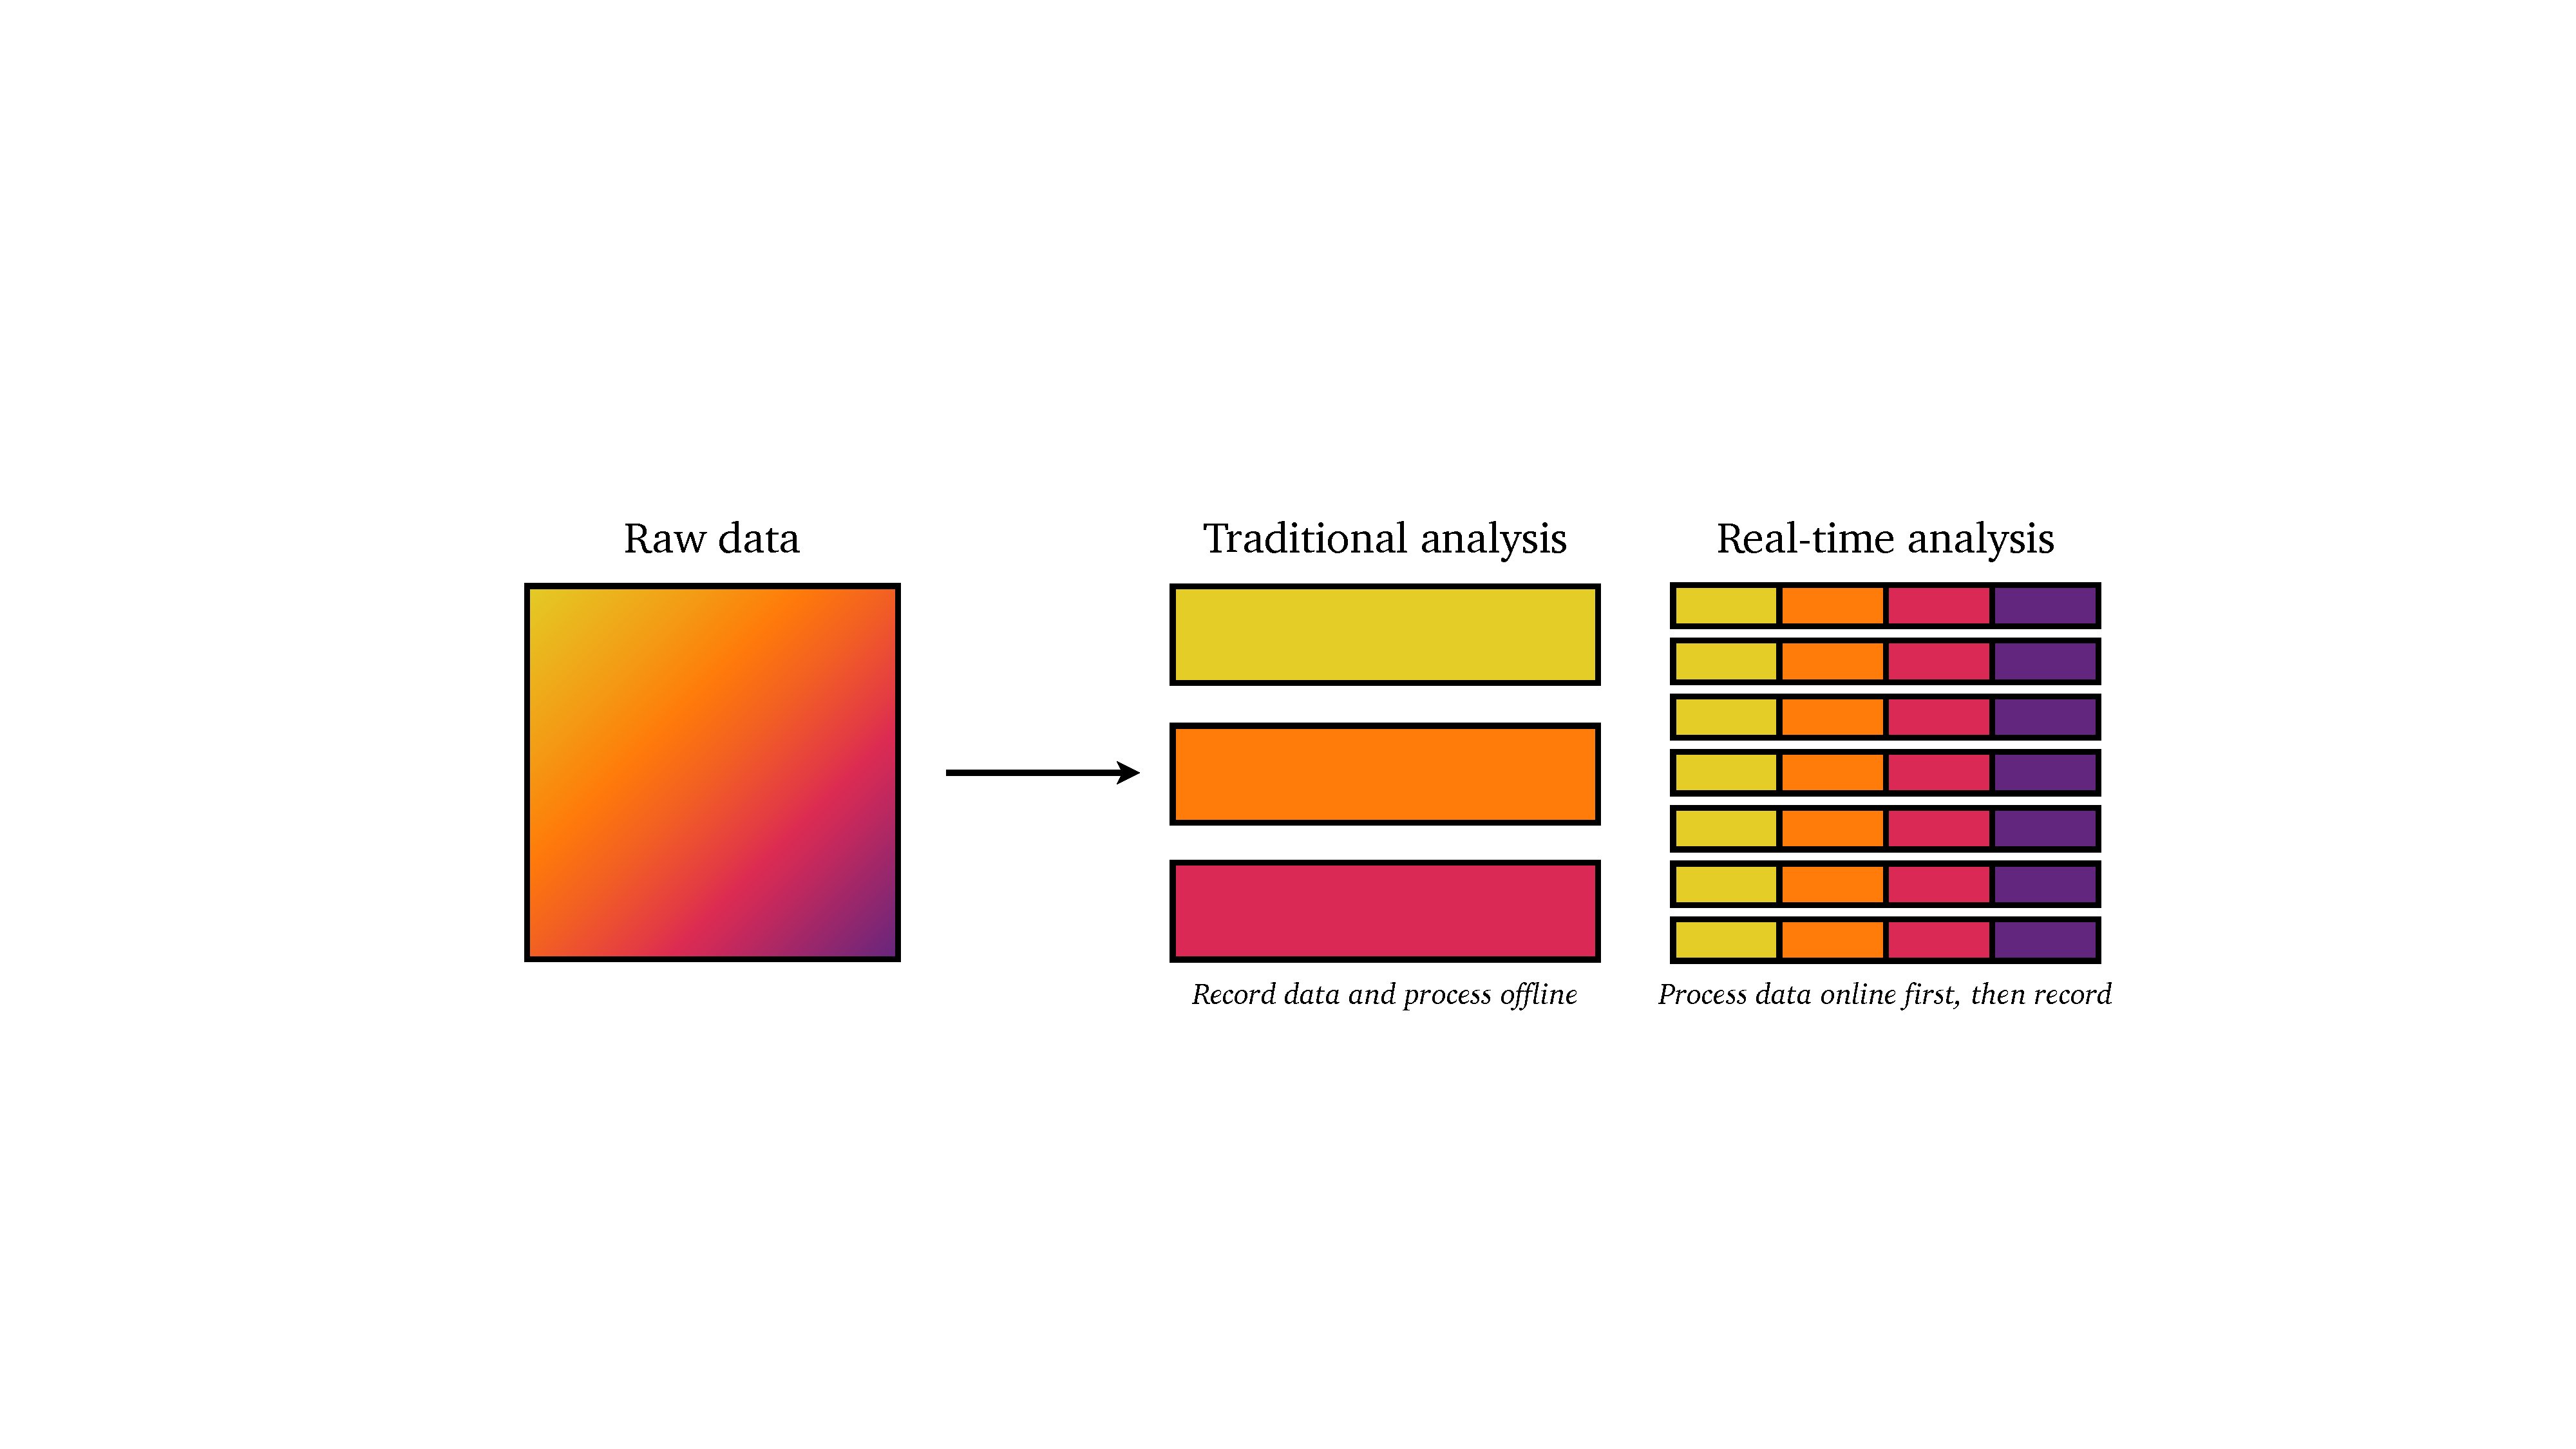
\includegraphics[width=\linewidth]{/Users/jgooding/Documents/SMARTHEP/CHEP2023/CHEP2023/proceedings/figures/rta-diagram.pdf}
    \caption{Traditional and RTA approaches to data processing. Traditional approaches rely on recording all data and processing this offline; in RTA, data is processed as it is produced, recording only the relevant portions, enabling greater volumes of processed data to be stored.}
    \label{rta-diagram}
\end{figure*}

RTA techniques have seen widespread adoption across HEP, in particular amongst trigger and data acquisition (TDAQ) systems. Since it is not possible to record a full detector readout and carry out event reconstruction at the LHC collision rate of {40}{ MHz}, triggers must be devised to select only those events relevant to the physics goals of an experiment. Such triggers conventionally consist of a hardware system making coarse decisions from partial detector readout, and a staged software trigger, applying gradually more finely-grained selections with increasingly more detailed reconstructions of events.

\subsection{Machine learning}
\label{machine-learning}
ML, a catch-all term for a family of techniques and technologies wherein algorithms are conditioned to analyse data, enables rapid decision-making and pattern recognition across a broad range of use cases~\cite{intro-ml}. In HEP, the adoption of ML began with classifiers for offline physics analysis, later widening to a variety of classification and pattern recognition/anomaly detection techniques for use online and offline~\cite{albertsson-ml}.

ML classifiers such as Boosted Decision Trees (BDTs) and Neural Networks (NNs) are commonly employed in HEP. The use of BDTs in signal selection for offline physics analysis has become standard practice, e.g., suppression of combinatorial background in the LHCb experiment measurement of the $B_s^0-\bar{B}_s^0$ oscillation frequency~\cite{delta-ms}. Classifiers can also aid tasks such as particle identification within event reconstruction, e.g., the CMS boosted event shape tagger, a NN trained to discriminate between possible $t$, $W^\pm$, $Z^0$ and $H$ candidates within an event~\cite{CMS-best}. ML classifiers also find many decision-making applications in industry, for example in the detection of malicious communications~\cite{classifier-phishing}.

ML techniques can also be applied to pattern recognition and anomaly detection—tasks which cannot otherwise be realistically performed on the scales of data presently being analysed. In industry, this is applied intuitively to fraud detection, wherein even subtle changes in transaction  data can indicate fraudulent activity~\cite{fraud-detection}. In HEP, such anomaly detection can be applied to searches, for example the ATLAS search for resonant decays to a Higgs boson~\cite{anomaly-hep}.

\subsection{Hybrid computing architectures}
\label{hybrid-architectures}
Central Processing Units (CPUs) have been used ubiquitously across many fields of research including HEP. CPUs are designed for general purpose computation (i.e., a single processor capable of performing a wide range of tasks with significant variety in computing/memory requirements), with large on-board memory and often multiple processing cores. However, recent advancements in computing have led to the development of accelerators, such as Graphical Processing Units (GPUs), Field-Programmable Gate Arrays (FPGAs), Application-Specific Integrated Chips (ASICs), etc. Accelerators are designed to perform specific tasks significantly faster than a CPU, by virtue of their structural design as represented in Figure~\ref{architectures}. A hybrid computing architecture is thereby a system formed of $2$ or more of the categories of processing units discussed: by designing the computing architecture around the nature of the tasks to be computed, computation can be significantly accelerated~\cite{architectures}.

\begin{figure*}[h!]
    \centering
    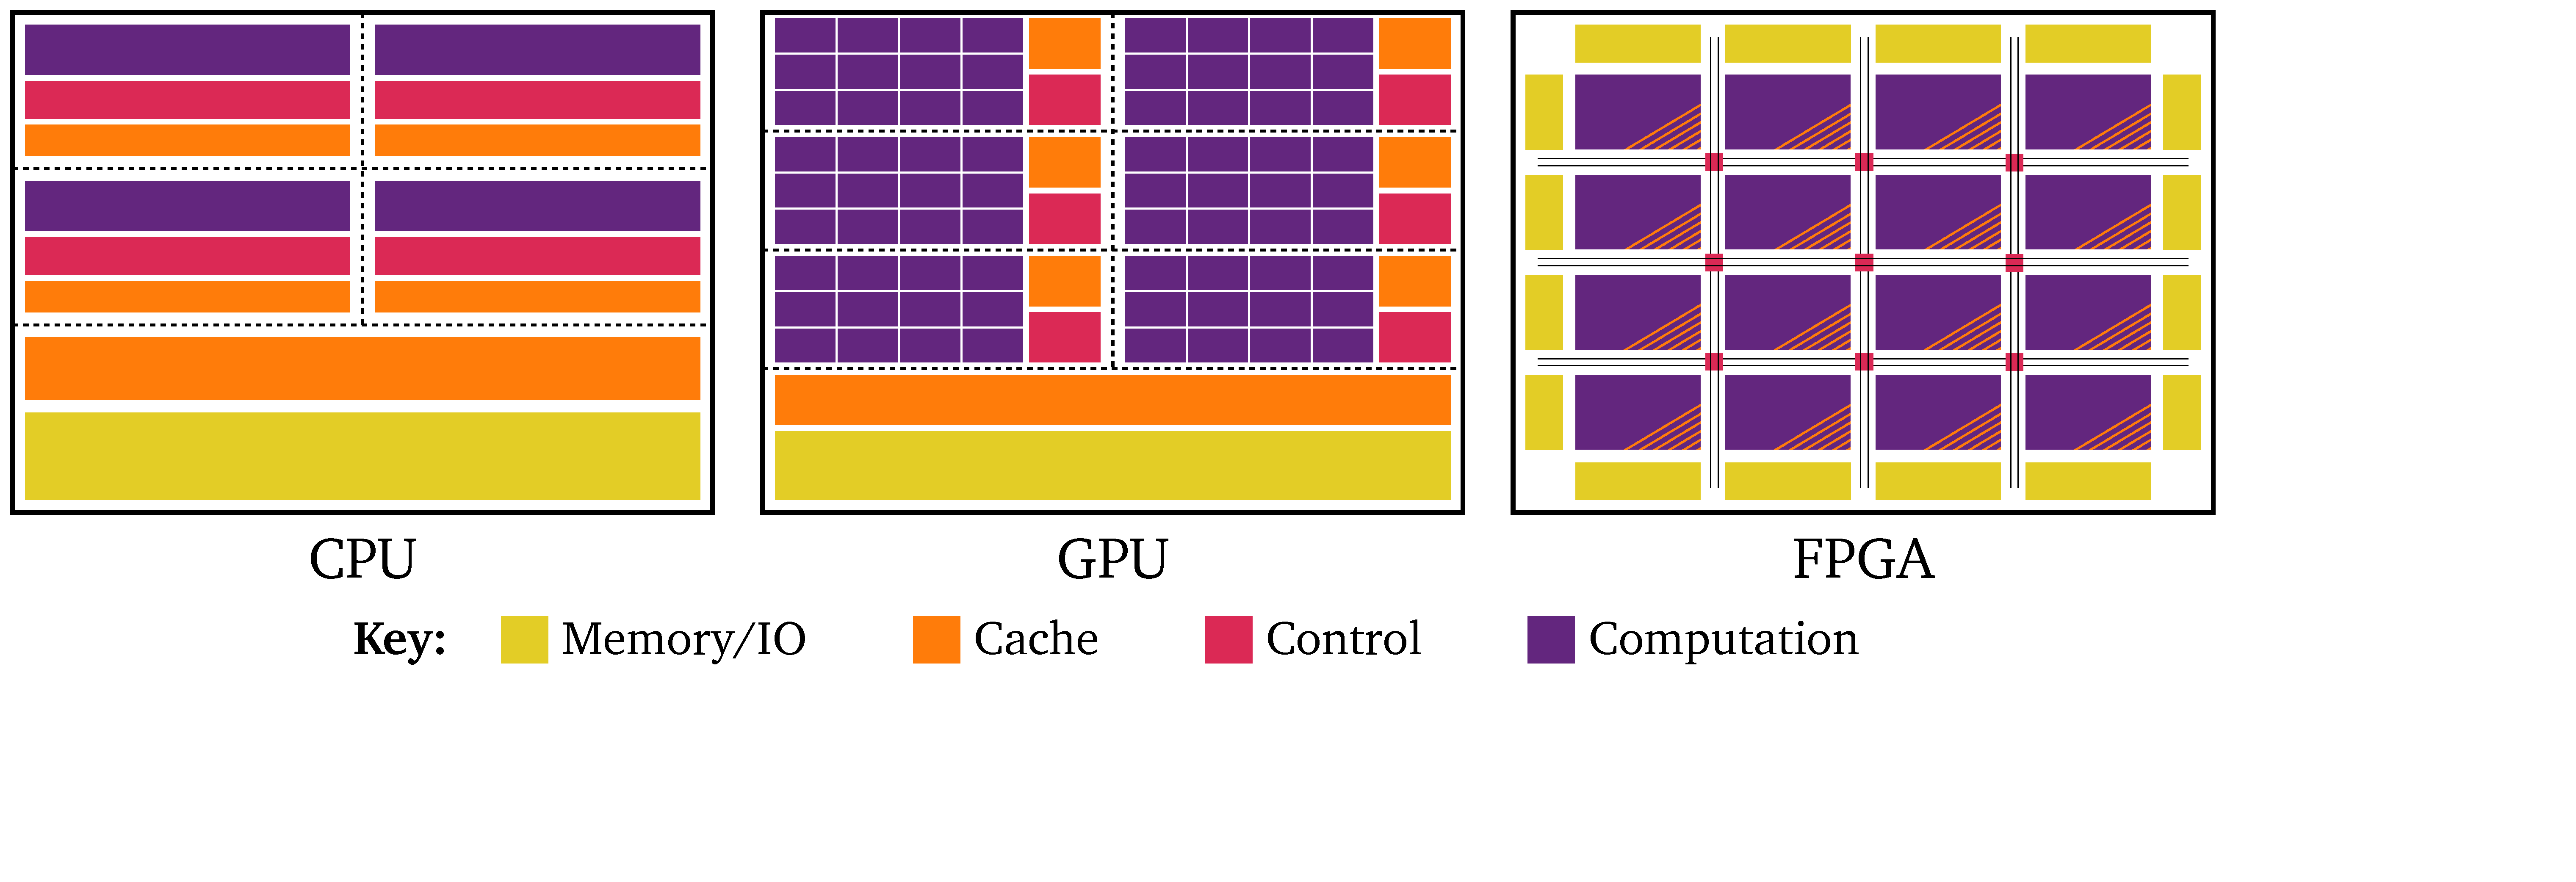
\includegraphics[width=\linewidth,clip]{/Users/jgooding/Documents/SMARTHEP/CHEP2023/CHEP2023/proceedings/figures/architectures-diagram.pdf}
    \caption{Comparison of CPU, GPU and FPGA architectures, illustrated as schematic diagrams. GPUs typically contain a greater proportion of computational resources than CPUs, with these resources subdivided within each multiprocessor to provide better parallel computing performance. FPGAs take a different approach, comprising many control blocks connected to memory/IO interface and to one another via switches~\cite{architectures}.}
    \label{architectures}
\end{figure*}

GPUs contain similar centralized resources to CPUs, but consist of many multiprocessors, each containing a greater proportion of computational resources than an equivalent CPU core. GPUs are thus well-suited to perform computationally intensive tasks in parallel, for example in event reconstruction at LHCb, where tasks such as track reconstruction and particle identification must be completed for every event~\cite{vomBruch-gpus}.

FPGAs are structured very differently, with memory and IO interface connected to many interlinked control blocks formed of simpler logic gate arrangements, often accompanied by a small cache. FGPAs are thus unable to complete complex tasks, though provide significant acceleration of simpler, highly parallelisable tasks. The programmable nature of FPGAs allows for their configuration with ML algorithms for fast performance~\cite{duarte-fpgas, muons-fpgas}.